\chapter{Grundlagen}

% Grundlagen:


% - TrackSort Schüttgutsortierung
% - Kalman Filter
% - NN
% 	- RNN
% 	- LSTM

\section{Das Kalman-Filter}
Als Kalman-Filter bezeichnet man ein mathematisches Verfahren mit dem Messfehler in realen Messwerten reduziert werden können und nicht messbare Systemgrößen geschätzt werden können. 


[vergangene, aktuelle und zukünftige Systemzustände schätzen]
[Einschränkung Linearität (Extended Kalman) und Gauß rauschen]

Der Zustand des Systems zum Zeitschritt $t$ wird als $y_t$ und die Messung im Zeitschritt $t$ als $z_t$ bezeichnet.

\begin{equation}
	y_t = A y_{t-1} + w, 	w \sim N(0, Q)
\end{equation}

\begin{equation}
	z_t = H y_{t} + v, 	v \sim N(0, R)
\end{equation}

Dabei ist $A$ die Zustandsübergangsmatrix, die den Übergang von einem Zustand in den nächsten beschreibt.
$H$ ist die Messmatrix, die beschreibt wie Messungen aus dem Zustand entstehen und Q und R sind die Kovarianzmatrizen des Systemrauschens beziehungsweise des Messrauschens. 

Das Kalman-Filter funktioniert mittels abwechselnd ausgeführter \textit{predict} und \textit{update} Schritte.

\begin{equation}
\hat{y}'_t = A \hat{y}'_{t-1}
\end{equation}

\begin{equation}
	\hat{P}'_t = A \hat{P}'_{t-1} A^\textit{T} + Q
\end{equation}




\section{Neuronale Netze}

Die Grundsteine des Feldes wurde 1943 von Warren McCulloch und Walter Pitts gelegt, 
die in ihrem Paper ein Neuronenmodell vorschlugen, mit dem sich logische arithmetische Funktionen berechnen lassen. 
Infolge dessen gab verschiedene Forschungsbestrebungen in dem Feld, wie [Examples: TODO!].

[Viele der Begrifflichkeiten, die wir heute noch verwenden wurden 1956 auf der Dartmouth Conference festlegt.]

Nachdem jedoch Marvin Minsky und Seymour Papert zeigten, dass einzelne Perzeptrons nicht in der Lage sind linear nicht separierbare Probleme zu lösen sank das Interesse an dem Feld.

\subsection{Perzeptron}
Die kleinste Einheit eines neuronalen Netzes ist das Perzeptron.
Es ist eine Art künstliches Neuron, dass eine Reihe an Eingaben entgegen nimmt und einen einzelnen Wert $o$ ausgibt.
Die einzelnen Eingaben $x_i$ haben jeweils eine Gewichtung $w_i$.
Es existiert ein sogenannter Schwellwert oder \textit{bias}, der normalerweise 
durch eine zusätzliche Eingabe $x_{m+1}$ mit dem Wert $+1$ und dem dazugehörigen Gewicht $w_{m+1}$ modelliert wird.
Den Ausgabewert $y$ erhält man dadurch, dass man die gewichteten Eingaben aufsummiert und in die Aktivierungsfunktion des Perzeptrons gibt.
Ein Überblick über verschiedene Aktivierungsfunktionen ist unter \ref{activationfuncs} zu finden.

Mathematisch ist die Ausgabe eines Perzeptrons also wie folgt definiert:

\begin{equation}
	y = \phi ( \sum_{i= 0}^{m} w_i x_i)
\end{equation}

Beim Lernen werden die Gewichte der einzelnen Eingaben so an gepasst, dass die gewünschte Ausgabe erreicht wird.
Ein einzelnes Perzeptron mit zwei Eingängen kann zur Darstellung der logischen Operatoren AND, OR und NOT genutzt werden

Letztendlich ist ein solches Perzeptron jedoch nur ein linearer Klassifikator und kann somit zum Beispiel den XOR Operator nicht auflösen.
Um solche, nicht linear-separierbare Probleme zu lösen müssen mehrere Schichten an Neuronen kombiniert werden.

\subsection{Aktivierungsfunktionen}
\label{activationfuncs}
Es gibt verschiedene Aktivierungsfunktionen, die für den Einsatz in neuronalen Netzen in Frage kommen.
Sie sind von essenzieller Wichtigkeit, da ohne eine Nicht-Linearität das Netz in eine einfache Regression kollabiert.

Eine Aktivierungsfunktion sollte leicht abzuleiten sein, 
da dies im Rahmen des Backpropagation Algorithmus häufig geschieht und sonst beträchtlicher Rechenaufwand entsteht.

Einige häufig verwendete Aktivierungsfunktionen sollen hier vorgestellt werden.
Jede dieser Funktionen stellt eine Nicht-Linearität dar und nimmt eine einzelne Zahl, wendet eine bestimmte, festgelegte mathematische 
Operation auf diese an und gibt das Ergebnis zurück.

\begin{description}
	\item[Sigmoid-Funktion] \hfill \\
		\begin{equation}
			f(x) = \frac{1}{1 + e^x} = \frac{e^x}{e^{x + 1}}
			\label{func:Sigmoid}
		\end{equation}
		\begin{equation}
			f'(x) = f(x) * (1 - f(x))
		\end{equation}
		Die mathematische Form der Sigmoid Aktivierungsfunktion ist in Abbildung \ref{sigmoidFunc} zu sehen.
		Sie bildet die reellen Zahlen $\mathbb{R}$ auf das Intervall $(0,1)$ ab. 
		Für betragsmäßig größer werdende negative Zahlen nähert sich der Rückgabewert $0$ an,
		ebenso wie für größer werdende positive Zahlen sich der Rückgabewert an $1$ annähert.

		Die Sigmoid Funktion ist eine historisch häufig genutze Funktion, da sie das Verhalten eines natürlichen Neurons,
		der biologischen Motivation für künstliche Neuronen, gut nachbildet:
		komplette Inaktivität eines Neurons bei Ausgabe 0 bis zum feuern mit maximaler Frequenz bei Ausgabe 1.

		In der Praxis jedoch haben sich einige Nachteile der Sigmoid Funktion gezeigt, weshalb sie quasi nicht mehr genutzt wird.
		Der gewichtigste von diesen ist, dass ihre Ableitung bei großen Beträgen beinah $0$ ist.
		Dies führt dazu, dass während der Ausführung des Backpropagation-Algorithmus beinah keine Änderungen passieren und dementsprechend das Netz sehr langsam lernt.
		
		\begin{figure}
			\centering
			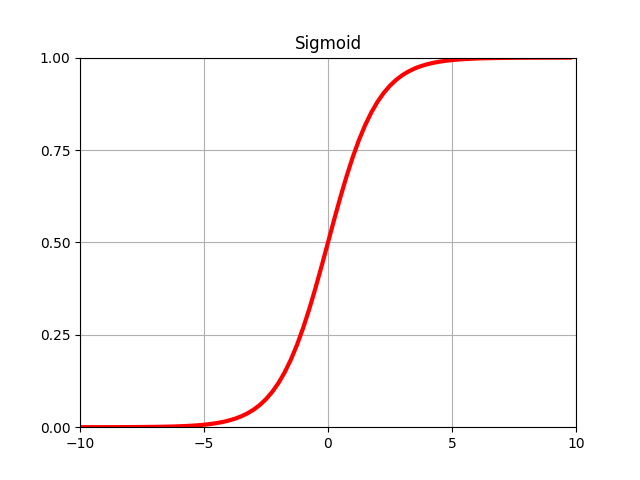
\includegraphics[width=0.618\textwidth]{Sigmoid}
			\caption{Plot der Sigmoid Funktion}
			\label{sigmoidFunc}
		\end{figure}
		  


	\item[TanH] \hfill \\
		\begin{equation}
			f(x) = tanh(x) = \frac{e^x - e^{-x}}{e^x + e^{-x}}
		\end{equation}
		\begin{equation}
			f'(x) = 1 - f(x)^2
		\end{equation}
		Die tanh Aktivierungsfunktion ist in Abbildung \ref{tanhfunction} dargestellt.
		Im Gegensatz zur Sigmoid Funktion bildet sie die reellen Zahlen $\mathbb{R}$ auf das Intervall $(-1, 1)$ ab.
		Weil sie zentriert um den Nullpunkt ist, wird sie bei realen Anwendungen der Sigmoid Funktion vorgezogen.
		Das Saturationsproblem der Sigmoid Funktion besteht jedoch immer noch.
		\begin{figure}
			\centering
			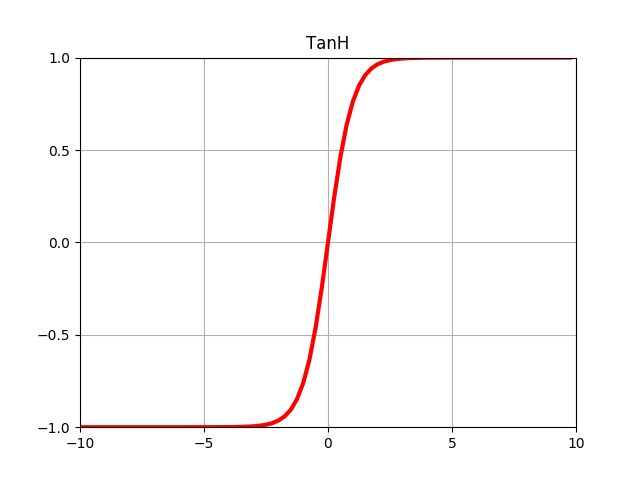
\includegraphics[width=0.618\textwidth]{Tanh}
			\caption{Plot der Tanh Funktion}
			\label{tanhfunction}
		\end{figure}
	
	\item[ReLU] \hfill \\
		\begin{equation}
			f(x) = max(0, x)
		\end{equation}
		\begin{equation*}
			f'(x) = \begin{cases}
			0 &\text{, falls $x < 0$}\\
			1 &\text{, falls $x > 0$}
			\end{cases}
		\end{equation*}
		Abbildung \ref{reluoutput} zeigt den Plot einer \textit{Rectified Linear Unit}, oder kurz ReLU.
		Die Aktivierung von ReLus ist ein einfacher Schwellwert, der weit weniger rechenintensiv ist, als die aufwendigen Exponenzialfunktionen von Sigmoid und tanh.
		In der Praxis hat sich gezeigt zudem gezeigt, dass ReLus deutlich schneller konvergieren als Sigmoid- oder tanh-Neuronen. 
		Krizhevsky et al. haben in ihrem Paper\cite{NIPS2012_4824} einen Geschwindigkeitsgewinn um Faktor 6 feststellen können.
		Ein Problem, das mit ReLUs jedoch existiert ist, dass einzelne Neuronen während dem Training "absterben" können.
		Diese Neuronen sind dann für jeden beliebigen Input inaktiv und können nie wieder etwas zur Ausgabe des Netzes beitragen.
		Durch die Wahl einer geeigneten Lernrate oder den Einsatz sogenannter Leaky ReLUs lässt sich dies jedoch vermeiden.
		

		\begin{figure}
			\centering
			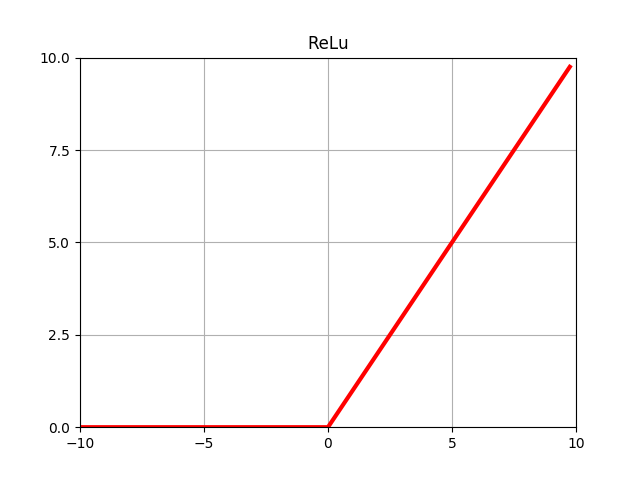
\includegraphics[width=0.618\textwidth]{ReLu}
			\caption{Plot der Ausgabe einer ReLUs}
			\label{reluoutput}
		\end{figure}



\end{description}

\begin{figure}[h]
    \centering
    \begin{subfigure}[t]{0.3\textwidth}
		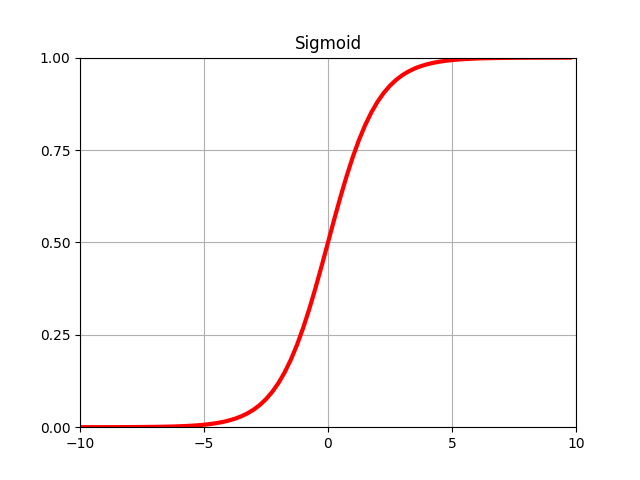
\includegraphics[width=\textwidth]{Sigmoid}
		\caption{Sigmoid Funktion}
    \end{subfigure}
    \begin{subfigure}[t]{0.3\textwidth}
		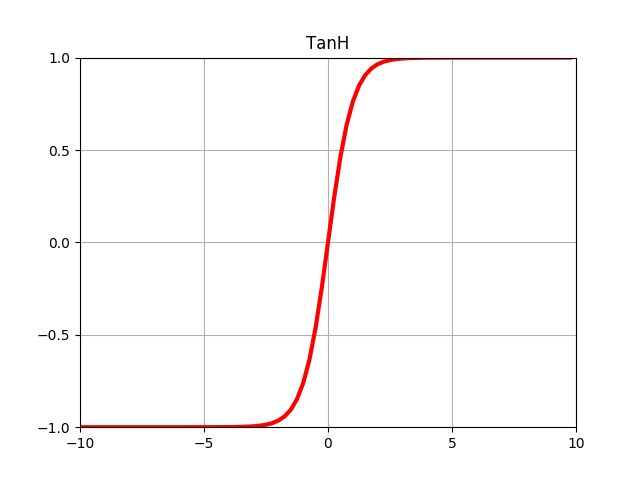
\includegraphics[width=\textwidth]{Tanh}
		\caption{TanH Funktion}
    \end{subfigure}
    \begin{subfigure}[t]{0.3\textwidth}
        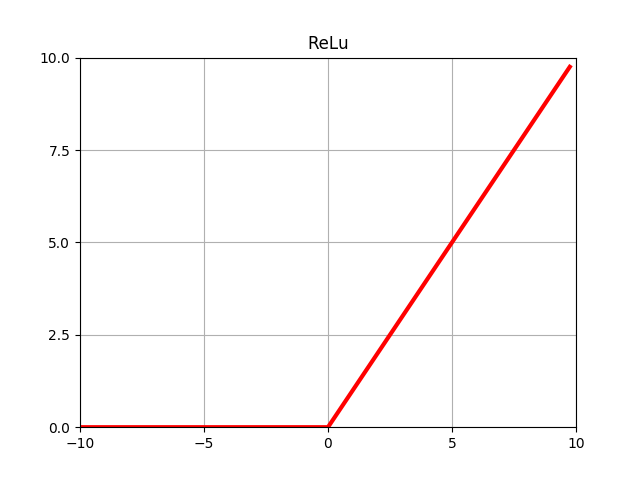
\includegraphics[width=\textwidth]{ReLu}
        \caption{ReLU}
    \end{subfigure}
    \caption{Häufig verwendete Aktivierungsfunktionen}
    \label{eval:function}
\end{figure}


\subsection{Feedforward Netze}

[eine absatz über Feedforward Netze. Basic]

\subsection{Backpropagation}

[ein Absatz über lernen mit dem Backpropagation Algorithmus]

\subsection{Rekurrente neuronale Netze}

[Text über rekurrente Netzwerke]